\documentclass{jarticle}
\usepackage{robomech}
\usepackage{graphicx}

\usepackage{mathrsfs}
\usepackage{bm}

\begin{document}
\makeatletter
\title{未知障害物環境に対応するための\\モンテカルロ自己位置推定における観測範囲の選択}
{―まだ決まってない―}
{Observation Range Selection in Monte Carlo localization for Unknown Obstacle Environments}
{-Not decided yet.-}

\author{
\begin{tabular}{ll}
 ○学\hspace{1zw} 池邉龍宏(千葉工大)& 正\hspace{1zw}林原靖男\hspace{1zw} (千葉工大)\\
 \hspace{1zw}正\hspace{1zw}上田隆一(千葉工大)\\
 % ※協賛・後援団体の会員資格で発表される場合は「正・学」は不要です。
 \end{tabular}
 % &\\
 \vspace{1zh} \\
 \begin{tabular}{l}
{\small Tatsuhiro IKEBE, Chiba Institute of Technology, 
 }\\
 {\small Yasuo HAYASHIBARA, Chiba Institute of Technology}\\
 {\small Ryuichi UEDA, Chiba Institute of Technology}\\
\end{tabular}
}
\makeatother

\abstract{ \small 
Not decided yet.
}

\date{} % 日付を出力しない
\keywords{Autonomous mobile robots, Navigation, LiDAR Localization, MCL, Unknown Obstacle}

\maketitle
\thispagestyle{empty}
\pagestyle{empty}


\section{緒言}%===========================

近年、自律移動ロボットの自己位置推定手法として、 Monte Carlo localization(MCL)\cite{MCL}
がよく用いられる。MCLは、ロボットの姿勢$\mathcal{X}$を多数のパーティクルで近似し、
推定した姿勢$\bm{x}$${ = (x, y, \Theta)}$を出力とするアルゴリズムである。
また、MCLはマルチモーダルな分布を持つことができ、割と強い自己位置推定だよー。
しかし、MCLのアルゴリズムでは、実環境に存在する未知障害物の対策は出来ていない。
そのため、未知障害物が存在する環境では、自己位置推定が破綻しやすい。
ここでいう未知障害物とは、ロボットが持っている地図(静的障害物)以外の障害物のことである。

 そのような環境の例としては、つくばチャレンジ\cite{つくばチャレンジ}が挙げられる。つくばチャレンジというのは、
実際に人や自動車が通る横断歩道、公園において、ロボットを約2km自律走行させる技術チャレンジです。
図\ref{fig: つくばチャレンジ人混み}は、つくばチャレンジのスタート地点である。
このような人混みがすごいような環境は、ロボットが持っている地図とLiDAR等の
センサから得られるデータとの照合の際に失敗する可能性が高い。
照合に失敗した場合、結果的にそれが原因で自己位置推定が破綻する。

 そのような問題に対応するためにいくつか研究がある。
xとyとzが存在する。xはこんな感じ、yはこんな感じ、zはこんな感じである。

 zの研究の未知障害物を観測に含めないことで、自己位置推定の破綻を防ぐということから
MCLのアルゴリズムレベルで対策を行うためのアイデアを得た。
そこで、本稿では、その性能について実験にて評価を行う。
2章では、未知障害物対策を実装したMCL、3章では実装したMCLの性能評価を行うための実験、
4章では結果から性評価を行い、最後に結言で本稿をまとめる。



\begin{figure}[h]
  \centering
   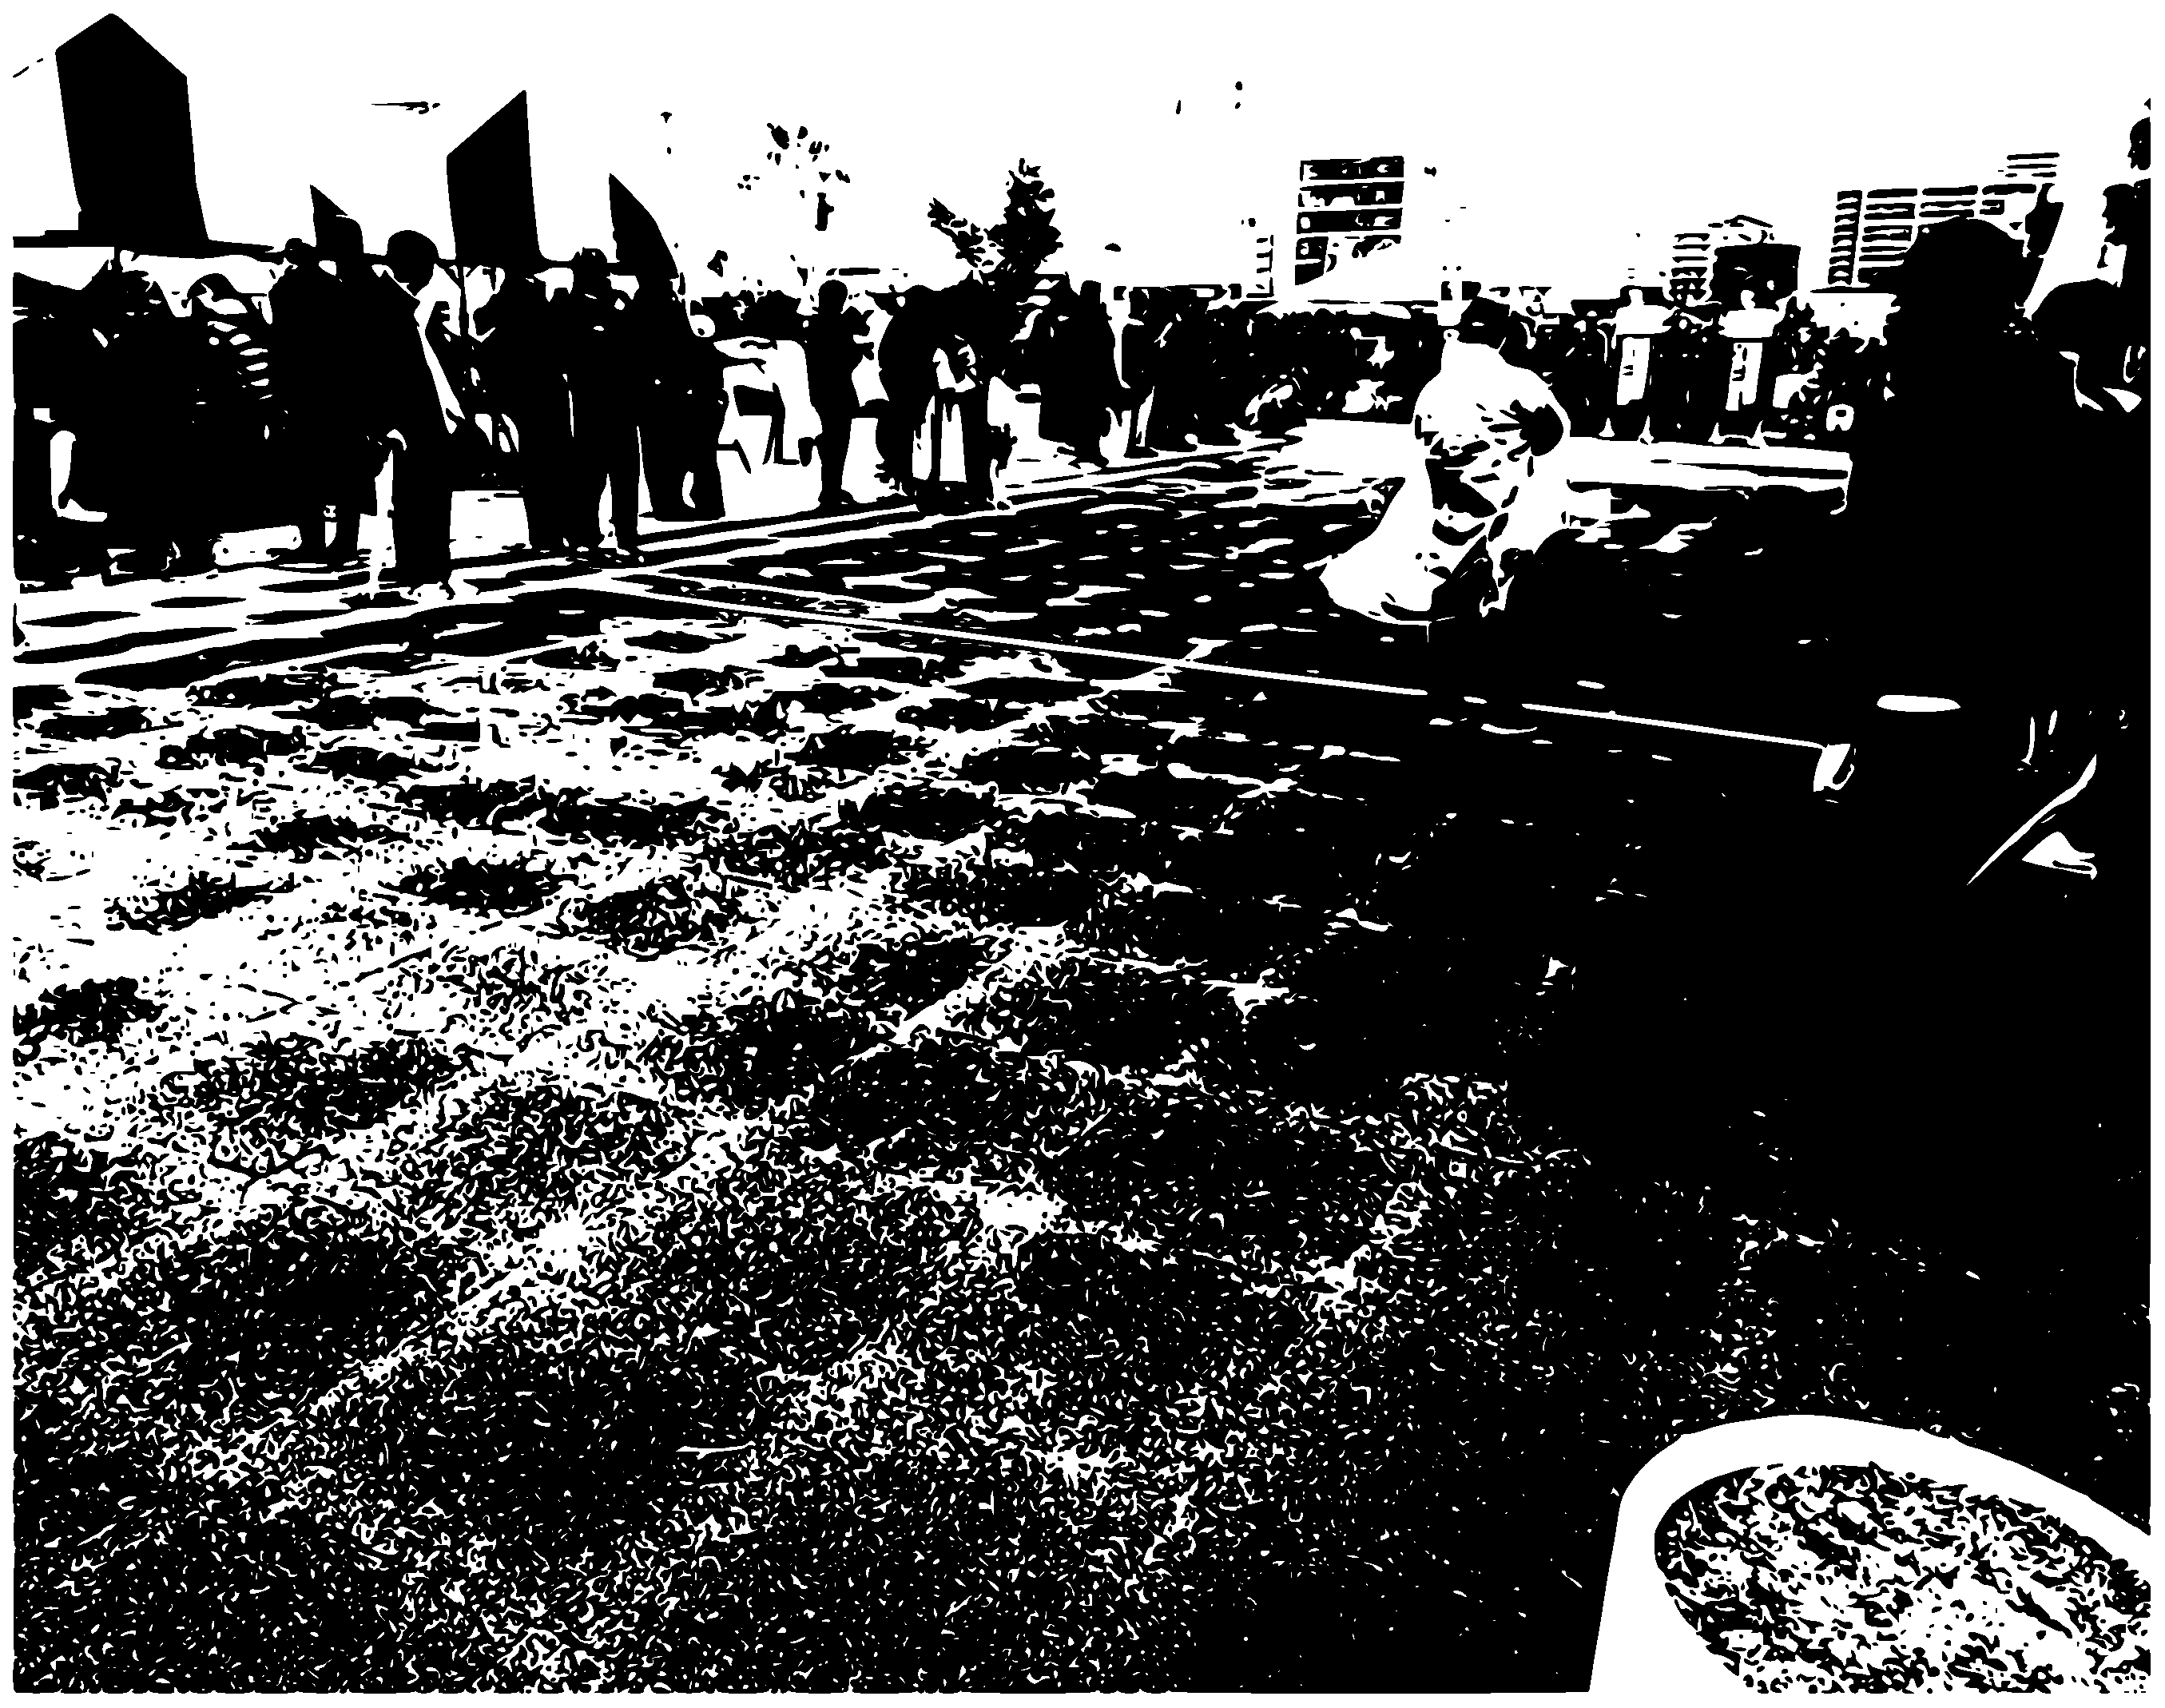
\includegraphics[height=38mm]{fig/hitogomi.eps}
   \vspace*{-4mm}
   \caption{Crowds at the start of the Tsukuba Challenge 2022}
   \label{fig: つくばチャレンジ人混み}
 \end{figure}

\section{手法}%===========================

% \subsection{}%-----------

\section{実験}%===========================

\section{実験結果}%===========================

\section{結言}%===========================


\footnotesize
\begin{thebibliography}{99}

\bibitem{MCL}

\bibitem{つくばチャレンジ}

\bibitem{Shinjuku99}

\end{thebibliography}

\normalsize
\end{document}
